\chapter{Opracowanie i~ocena eksperymentalna klasyfikatora intencji użytkownika} \label{sec:klasyfikator}
\label{chapters:05-Klasyfikator_intencji}

\section{Wyzwania interpretacji semantycznej poleceń użytkownika}

Głównym celem projektowanego modułu \definicja{Asystenta NLP} w systemie \definicja{Moje Konie} jest umożliwienie użytkownikowi, najczęściej hodowcy koni lub pracownikowi stajni, interakcji z systemem za pomocą języka naturalnego. 

Jak wskazuje w swoich pracach Christopher Manning \cite{manning2008}, współczesne wyzwanie w przetwarzaniu języka naturalnego (NLP) przesunęło się z prostego rozpoznawania słów w stronę głębokiego rozumienia intencji i kontekstu, co jest kluczowe dla budowy systemów zdolnych do realnej pomocy człowiekowi w konkretnych dziedzinach życia.

W specyficznych warunkach pracy terenowej, takich jak stajnia czy padok, tradycyjne wprowadzanie danych poprzez formularze webowe jest często niepraktyczne. Rozwiązaniem jest interfejs konwersacyjny (czat lub komendy głosowe), który przekłada swobodną wypowiedź na ustrukturyzowane żądanie do bazy danych. Zadanie to wymaga od systemu nie tylko rozpoznania fonetycznego lub tekstowego, ale przede wszystkim precyzyjnego przypisania wypowiedzi do odpowiedniej akcji w systemie (\english{Intent Classification}).

\subsection*{Definicja problemu mapowania intencji}

System musi być zdolny do poprawnej interpretacji i przekierowania zapytania do jednego z~ośmiu predefiniowanych obszarów funkcjonalnych (końcówek REST API), obsługujących zarządzanie hodowlą:
\begin{description}
    \item[Zarządzanie stadem:] rejestracja i edycja koni (\texttt{/api/konie}).
    \item[Rozród:] ewidencja kryć, wyźrebień i kontroli weterynaryjnej rozrodu (\texttt{/api/wydarzenia/rozrody}).
    \item[Profilaktyka:] odnotowywanie szczepień, odrobaczania, suplementacji czy wizyt dentystycznych (\texttt{/api/wydarzenia/zdarzenia\_profilaktyczne}).
    \item[Pielęgnacja kopyt:] dokumentowanie wizyt kowala i zabiegów werkowania (\texttt{/api/wydarzenia/\allowbreak{}podkucie}).
    \item[Weterynaria i zdrowie:] monitorowanie procesów leczenia (\texttt{/api/wydarzenia/leczenia}), diagnozowanie chorób (\texttt{/api/wydarzenia/choroby})
    \item[Baza kontaktów:] zarządzanie bazą kontaktów do specjalistów (\texttt{/api/kowale}, \texttt{/api/weterynarze}).
\end{description}

\subsection*{Trudności w przetwarzaniu języka naturalnego (NLP)}

Zrozumienie intencji użytkownika w tym konkretnym przypadku napotyka na bariery, które w~literaturze przedmiotu uznaje się za kluczowe problemy NLU (\textit{Natural Language Understanding})~\cite{jurafsky2023}:

\begin{description}
    \item[Zróżnicowanie lingwistyczne i semantyczne:] Użytkownicy używają różnych konstrukcji dla tej samej czynności (np. ,,Kasztanka została zaszczepiona'' vs ,,Dodaj szczepienie dla Kasztanki''). Zgodnie z tezą Manninga \cite{manning2008}, system musi tu wykazać się zdolnością rozumienia, by odwzorować oba sformułowania na właściwą końcówkę profilaktyki.
    
    \item[Specjalistyczna terminologia:] Branża jeździecka operuje słownictwem (np. ,,werkowanie'', ,,źrebność''), które rzadko występuje w korpusach języka ogólnego, co wymaga od modelu wysokiej jakości reprezentacji wektorowych (\english{embeddings}) zdolnych do uchwycenia relacji między tymi terminami a ich medycznym znaczeniem.
\end{description}

\section{Ewolucja architektury: od modelu monolitycznego do podejścia hybrydowego}

W początkowej fazie projektowania systemu asystenta, proces interpretacji zapytania opierał się na architekturze monolitycznej z wykorzystaniem dużych modeli językowych (LLM). W tym podejściu surowy tekst użytkownika był przesyłany bezpośrednio do modelu (np. Gemini lub DeepSeek) wraz z pełną dokumentacją wszystkich ośmiu dostępnych punktów końcowych API w~jednym zapytaniu. Zadaniem modelu było jednoczesne rozpoznanie intencji oraz wygenerowanie poprawnie sformatowanego obiektu JSON, służącego jako ciało żądania HTTP.

\subsection{Ograniczenia podejścia monolitycznego}

Wstępne testy wykazały, że mimo wysokiej elastyczności modeli LLM, takie rozwiązanie posiada istotne wady z punktu widzenia wydajności systemu:

\begin{description}
	\item[Nadmiarowość kontekstu:] Dołączanie pełnego schematu API (wszystkich ośmiu końcówek) do każdego zapytania drastycznie zwiększało liczbę tokenów wejściowych. Generuje to nieuzasadnione koszty operacyjne, zwłaszcza przy częstym korzystaniu z płatnych API, oraz zwiększa czas oczekiwania na odpowiedź \cite{liu2023}, a~zatem takie rozwiązanie nie jest skalowane do większych systemów.
    
	\item[Szum informacyjny:] Przekazywanie do modelu informacji o końcówkach niezwiązanych z danym zapytaniem (np. schemat rozrodu przy pytaniu o kowala) zwiększa ryzyko halucynacji. Model, mając zbyt szeroki kontekst, może próbować odwzorowywać dane do niewłaściwych pól, co obniża ogólną precyzję żądania.
    
	\item[Trudność w debugowaniu:] Przy podejściu ,,wszystko w jednym'', trudno jest jednoznacznie określić, czy błąd wynika z błędnego rozpoznania intencji, czy z problemów modelu ze zbudowaniem poprawnego obiektu JSON.
\end{description}

\subsection{Przejście na model hybrydowy}

Zdecydowano się na zmianę architektury na model hybrydowy, w którym proces przetwarzania zapytania został rozdzielony na dwa etapy. Pierwszym krokiem jest wykorzystanie dedykowanego, ,,lekkiego'' klasyfikatora opartego na osadzeniach wektorowych (\english{word/sentence embeddings}), którego jedynym zadaniem jest identyfikacja intencji użytkownika.
Głównym założeniem tej zmiany było przeniesienie ciężaru klasyfikacji na lokalny lub tańszy w~eksploatacji model wektorowy, co pozwoliło na:

\begin{description}
	\item[Dynamiczne budowanie zapytania:] Do modelu LLM wysyłany jest wyłącznie ten fragment dokumentacji API, który jest bezpośrednio związany z intencją wykrytą przez klasyfikator. Takie podejście, znane jako \textit{context pruning}, pozwala na redukcję rozmiaru zapytania o~znaczący procent, co przekłada się na realne oszczędności tokenów \cite{jimenez2022}.
    
	\item[Większą precyzję odwzorowania:] Model LLM, otrzymując instrukcję dotyczącą tylko jednej, konkretnej końcówki, rzadziej popełnia błędy w~odwzorowaniu pól technicznych i lepiej radzi sobie z ekstrakcją parametrów z tekstu.
    
	\item[Separację logiki:] Wyodrębnienie klasyfikatora pozwoliło na precyzyjne dostrajanie procesu wykrywania intencji (np. poprzez wykorzystanie algorytmu k-NN i doborze jego hiperparemetrów) niezależnie od warstwy generatywnej.
\end{description}

Wdrożenie tej separacji umożliwiło nam zbadanie, jak klasyczne metody uczenia maszynowego operujące na wektorach semantycznych radzą sobie z branżowym słownictwem.
Nasz problem jednak wciąż wiązał się z:

\begin{description}
    \item[Niejasnością i skrótowością:] Krótkie komunikaty wysyłane w pośpiechu (np. ,,kowal u Gwiazdy'') wymuszają na systemie automatyczne rozpoznanie, że chodzi o wizytę kowala i przypisanie jej do konkretnego konia, co bez zrozumienia kontekstu branżowego byłoby niemożliwe.
    \item[Ekstrakcją encji:] Poza samą intencją, system musi ,,wyłowić'' z tekstu kluczowe parametry (np. imię konia, datę, nazwę leku), by stworzyć poprawne żądanie POST do API.
\end{description}

W związku z powyższym, proste dopasowanie słów kluczowych okazało się niewystarczające. Zdecydowaliśmy się stworzyć architekturę, która połączy elastyczność dużych modeli językowych (LLM) z precyzją i wydajnością klasyfikatorów wektorowych. Klasyfikator wektorowy został przeznaczony do rozwiązania problemu klasyfikacji intencji, a na LLM została zrzucona cała odpowiedzialność wypełnienia żądania mając już informacje o końcówce.

\section{Metodyka i implementacja klasyfikatora intencji}

Fundamentem działania nowoczesnych systemów rozumienia tekstu jest transformacja symboli językowych na gęste reprezentacje wektorowe w przestrzeni wielowymiarowej. W projektowanym systemie proces ten realizowany jest za pomocą zaawansowanego modelu osadzeń słów (\english{embeddings}) \texttt{multilingual-e5-large-instruct}, który opiera się na architekturze transformatora.

W przeciwieństwie do tradycyjnych metod, takich jak Bag-of-Words czy TF-IDF, które bazują na częstotliwości występowania słów, modele oparte na osadzeniach kodują relacje semantyczne i kontekstualne. Model E5 generuje wektory o stałej długości 1024 komponentów, co pozwala na uchwycenie subtelnych różnic znaczeniowych między zapytaniami.

Wykorzystanie wariantu ,,instruct'' wprowadza dodatkową warstwę precyzji -- system wymaga stosowania prefiksów instrukcyjnych (np. \texttt{query:} dla danych wejściowych użytkownika oraz \texttt{passage:} dla wzorców w bazie wiedzy). 
Taka asymetria w procesie wektoryzacji jest kluczowa dla efektywnego mapowania krótkich, często niekompletnych pytań na opisy funkcji systemowych zawarte w~dokumentacji API \cite{reimers2019}.

W praktycznej implementacji proces ten opiera się na dwóch niezależnych strumieniach danych, integrowanych w wspólnej przestrzeni wektorowej. Pierwszym z nich jest dynamiczne zapytanie użytkownika (\textit{query}), czyli surowa wypowiedź naturalna, która po procesie normalizacji jest zamieniana na wektor . Drugim elementem jest statyczna baza wiedzy, składająca się w bieżącej wersji systemu z 480 zdefiniowanych przykładów (\textit{passages}), reprezentujących wzorcowe sformułowania dla poszczególnych intencji.

Poniższy przykład ilustruje strukturę przygotowania danych przed ich wektoryzacją, prezentując transformację zapytania użytkownika o nowym koniu oraz fragment bazy 480 wzorców:

\begin{verbatim}
# 1. STRUMIEŃ ZAPYTANIA (Query) - wypowiedź użytkownika
"query: dodaj nowego konia blyskawica to 6 letnia klacz wlasnie ja przywiozlem"

# 2. STRUMIEŃ BAZY WIEDZY (Passages) - wybrane z 480 przykładów
"passage: chce dodac mloda klacz kore do hodowli"
"passage: prosze wprowadzic nowego konia brego kon rekreacyjny czteroletni"
"passage: dodaj do mojej stajni 6 letniego ogiera zenita"
"passage: dopisz konia neptuna mlodego walacha do jazdy terenowej"
"passage: zarejestruj w hodowli klacz melodie 3 lata"
\end{verbatim}



Zastosowana asymetria pozwala na obliczenie podobieństwa cosinusowego między wektorem zapytania a każdym z wektorów bazy. Dzięki semantycznemu kodowaniu modelu E5, system potrafi zidentyfikować, że potoczna fraza „właśnie ją przywiozłem” w połączeniu z opisem zwierzęcia odpowiada intencji rejestracji nowego obiektu, wykazując najwyższą korelację z przykładami takimi jak „wprowadź nowego konia” czy „dopisz konia do stajni”.



\subsection*{Baza wiedzy i kotwice}

Skuteczność klasyfikacji w systemach dedykowanych dziedzinowo jest nierozerwalnie związana z~jakością bazy wiedzy, która pełni rolę semantycznego układu odniesienia. W ramach implementacji przygotowano zestaw wzorcowych intencji, z których każda odpowiada jednej z ośmiu końcówek API. Każda intencja reprezentowana jest przez zestaw tzw. kotwic (\english{anchors}) -- starannie dobranych sformułowań, które modelują typowy sposób komunikacji użytkownika. Proces ten można przyrównać do nadzorowanego uczenia maszynowego typu \textit{few-shot learning}, gdzie system uczy się rozpoznawać kategorie na podstawie ograniczonej liczby przykładów.

Zastosowanie {dużych modeli językowych} (\akronim{LLM}) sprawia dodatkowo, że system wykazuje się wysoką odpornością na błędy gramatyczne oraz zapożyczenia, co w specyficznym języku hodowców koni, łączącym potoczne sformułowania z branżową terminologią specjalistyczną, ma fundamentalne znaczenie \cite{wang2022}.

\subsection*{Ewolucja algorytmu: od k-NN do centroidów}

W dążeniu do poprawy zdolności klasyfikatora do generalizacji, ewolucja algorytmu decyzyjnego zakładała przejście od analizy punktowej do modelowania uśrednionego rozkładu kategorii. Pierwotnie zaimplementowany algorytm K-Najbliższych Sąsiadów (k-NN) dla $k=1$ charakteryzował się dużą czułością na jednostkowe sformułowania wzorcowe.

Jako istotną poprawkę zaproponowano klasyfikację opartą na centroidach kategorii. W tym modelu każda z ośmiu intencji reprezentowana jest przez pojedynczy wektor centroidu $C_i$, obliczany jako średnia arytmetyczna wszystkich wektorów wzorcowych danej klasy, zgodnie ze wzorem (\ref{eq:centroid}).

\begin{equation}
    C_i = \frac{1}{N} \sum_{j=1}^{N} v_{i,j}
    \label{eq:centroid}
\end{equation}

\noindent gdzie:
\begin{itemize}
    \item $C_i$ -- wektor centroidu odpowiadający $i$-tej intencji,
    \item $v_{i,j}$ -- $j$-ty wektor wzorcowy należący do intencji $i$,
    \item $N$ -- liczba wektorów wzorcowych przypisanych do danej intencji.
\end{itemize}

Celem tej modyfikacji było wyznaczenie stabilnego „środka ciężkości” dla każdej operacji dostępnej w interfejsie API. W tak zdefiniowanej przestrzeni metrycznej, proces decyzyjny klasyfikatora polega na wyznaczeniu miary podobieństwa cosinusowego między wektorem zapytania użytkownika $q$ a wszystkimi centroidami $C_i$. Ostateczna klasyfikacja dokonywana jest poprzez wybór intencji, która wykazuje najwyższą wartość tego podobieństwa, co można zapisać za pomocą operatora argumentu maksymalizującego:

\begin{equation}
    \text{intent} = \arg\max_{i} \left( \frac{q \cdot C_i}{\|q\| \|C_i\|} \right)
\end{equation}

Podejście to pozwoliło na zredukowanie wpływu szumu informacyjnego oraz wyeliminowanie problemu nadmiernej czułości na odosobnione, nietypowe sformułowania znajdujące się w bazie wzorców. Dzięki uśrednieniu reprezentacji wektorowych, model zyskał wyższą zdolność do generalizacji, skupiając się na kluczowych cechach semantycznych wspólnych dla całej grupy 480 przykładów definiujących logiczne punkty końcowe systemu.

\subsection*{Logika decyzyjna i progi pewności}

Krytyczna analiza zachowania modelu pozwoliła na uproszczenie logiki decyzyjnej poprzez rezygnację z pierwotnie planowanych progów pewności (\english{confidence thresholds}), które zmuszały klasyfiakator do analizowania słów kluczowych. Doświadczenia wykazały jednak, że model osiąga skrajnie niskie wartości podobieństwa niemal wyłącznie w sytuacjach, gdy wprowadzony tekst jest zupełnie pozbawiony informacji semantycznych co przekłada się na niemożność zbudowania poprawnego zapytania w póżniejszym etapie. W sytuacjach, gdy użytkownik formułuje jakąkolwiek intencję związaną z domeną systemu, model z dużą precyzją wskazuje właściwy kierunek semantyczny.

\section{Benchmarking i optymalizacja}

\subsection{Dane użyte w eksperymencie}

W celu empirycznego wyznaczenia optymalnej konfiguracji dla systemu \definicja{Moje Konie}, przeprowadzono serię testów ewaluacyjnych. Do eksperymentu przyjęto zbiór danych podzielony na:
\begin{description}
	\item[Bazę wiedzy:] 60 reprezentatywnych przykładów, pełniących funkcję kotwic (\english{anchors}).
	\item[Zbiór testowy:] 40 unikalnych, nieznanych modelowi przykładów.
\end{description}

Dane były generowane ręcznie przez uczestników projektu, którzy na podstawie swojego doświadczenia z hodowcami koni próbowali odtworzyć ich sposób mówienia, jednocześnie zapewniając, że przykłady spełniają podstawowe wymagania systemu. Zależało nam, że nasz zbiór danych pokrywał różny poziom formalności przekazywanai informacji stąd np. w końcówce \texttt{api/wydarzenia/\allowbreak{}rozrody} znajdują się przykłady takie jak:

\begin{itemize}
    \item ,,Dino miał dzisiaj sprawdzanie źrebności. Alicja powiedziała, że wszystko było ok'',
    \item ,,Dodaj proszę informację, że klacz Bella była dziś inseminowana przez dr Kowalską'',
    \item ,,Wczoraj Tomek podkuł Lasera''.
\end{itemize}
Dane zostały przygotowane w formacie JSON, gdzie dla każdej końcówki przypisana jest lista zdań.

\subsection{Metodyka benchmarkingu hiperparametru sąsiedztwa}

Kluczowym aspektem strojenia modelu opartego na algorytmie k-NN  jest dobór odpowiedniej wielkości sąsiedztwa $k$, która determinuje strefę wpływu lokalnego na decyzję klasyfikacyjną \cite{manning2008}.
Ewaluację przeprowadzono dla zmiennych wartości $k$, mierząc skuteczność za pomocą metryk: dokładność (\english{accuracy}) oraz F1-makro. Wybór F1-makro był podyktowany koniecznością równoprawnego traktowania wszystkich intencji.

\subsection*{Strategia rozstrzygania remisów}

W klasycznym algorytmie k-NN dochodzi do sytuacji spornych, gdzie dwie lub więcej klas otrzymują identyczną liczbę głosów. W badanej implementacji zastosowano heurystykę opartą na gęstości semantycznej. W przypadku remisu głosów, ostateczna predykcja $y_{pred}$ jest wybierana na podstawie sumy podobieństw cosinusowych sąsiadów należących do danej klasy:

\begin{equation}
    y_{pred} = \argmax_{c \in C_{tied}} \left( \sum_{i \in N_c} \cos(\vec{x}, \vec{x}_i) \right)
\end{equation}
%
gdzie $N_c$ to zbiór sąsiadów należących do spornej klasy $c$, a $\vec{x}$ to wektor zapytania. Takie podejście premiuje klasę, której przykłady znajdują się ,,semantycznie bliżej'' zapytania użytkownika.
W~ramach eksperymentu przeprowadzono ewaluację algorytmu k-NN dla wartości parametru $k$~w~zakresie od 1 do 20 dla pełnego zbioru danych. Wyniki uzyskane dla zbioru testowego przedstawiono na Rysunku~\ref{fig:knn_eval}.

\begin{figure}%[H]
    \centering
    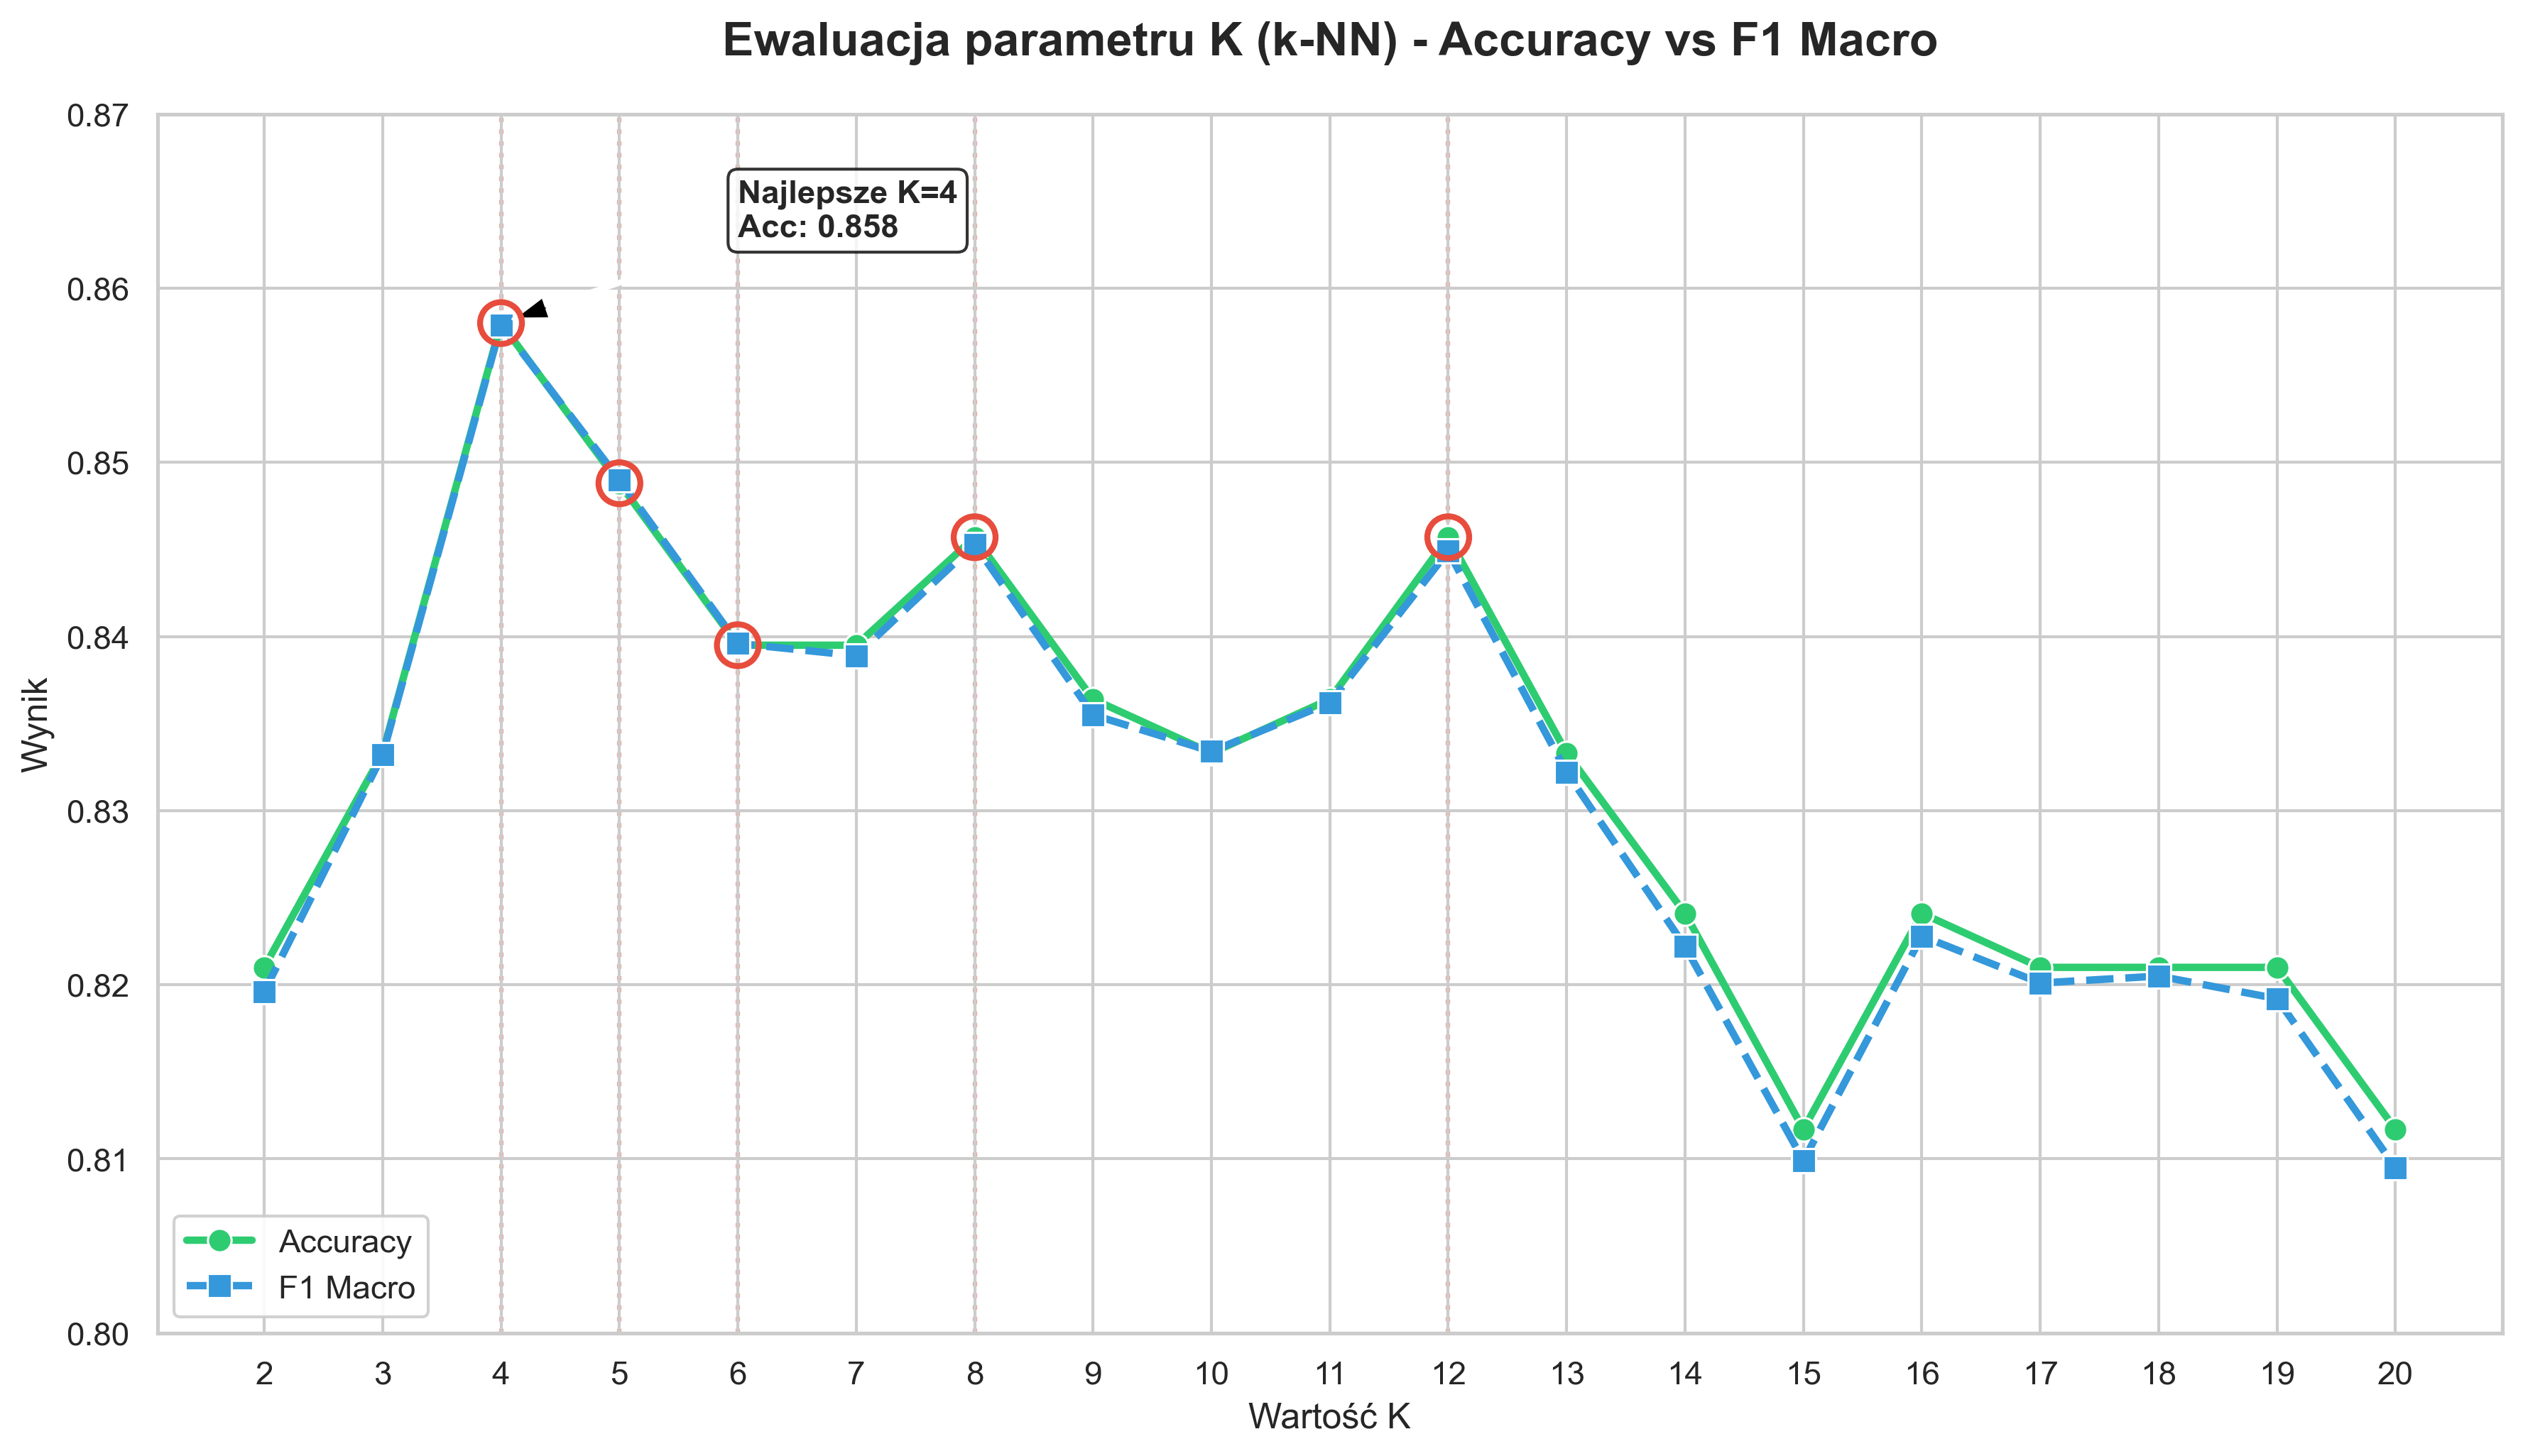
\includegraphics[width=0.9\textwidth]{public/wykres_knn.png} 
    \caption{Ewaluacja parametru k (k-NN) -- dokładność (\english{accuracy}) oraz F1-makro (\english{F1-macro}). Najlepsze wyniki uzyskano dla $k=4$.
    Czerwonymi okręgami zaznaczono pięć najlepszych wyników pod względem dokładności.}
    \label{fig:knn_eval}
\end{figure}

% TODO - wykres jako wykres + odwołania i opis
% TODO - tabelka jako tabelka

Eksperyment wykazał, że najwyższą dokładność uzyskano dla parametru $k \in \{4, 5, 6, 8, 12\}$. Należy jednak zaznaczyć, że rozpiętość wyników dokładności wyniosła ok. $0{,}05$, co przy ograniczonej liczebności zbioru testowego ($40$ przykładów na końcówkę) nakazuje zachować ostrożność w~interpretacji istotności tych różnic. 

Dodatkowo, dla tego samego zbioru danych, zweryfikowano podejście oparte na centroidach. Metoda ta niespodziewanie osiągnęła najwyższe wyniki zarówno pod względem dokładności, jak i~miary F1, co przedstawiono w Tabeli~\ref{tab:top_configurations}.

\begin{table}[H]
    \centering
    \caption{6 najlepszych konfiguracji wg. dokładności.}
    \label{tab:top_configurations}
    \begin{tabular}{|c|c|c|}
        \hline
        \textbf{k} & \textbf{dokładność} & \textbf{F1-makro} \\ 
        \hline
        centroid & $0{,}8735$ & $0{,}8736$ \\ 
        \hline
        4 & $0{,}8580$ & $0{,}8579$ \\ 
        \hline
        5 & $0{,}8488$ & $0{,}8490$ \\ 
        \hline
        8 & $0{,}8457$ & $0{,}8453$ \\ 
        \hline
        12 & $0{,}8457$ & $0{,}8449$ \\ 
        \hline
        6 & $0{,}8395$ & $0{,}8396$ \\ 
        \hline
    \end{tabular}
\end{table}

\subsection{Regularyzacja modelu poprzez zespołowe głosowanie}

W uczeniu maszynowym regularyzacja jest procesem wprowadzania dodatkowych ograniczeń w celu zapobiegania przeuczeniu (\english{overfitting}) i poprawy zdolności modelu do generalizacji \cite{goodfellow2016}. W kontekście modeli opartych na sąsiedztwie ryzyko to objawia się dwojako:

\begin{itemize}
    \item Dla małych wartości $k$ (np. $k=1$), model wykazuje wysoką wariancję i jest nadmiernie wrażliwy na szum.
    \item Dla dużych wartości $k$, następuje wzrost obciążenia (\textit{bias}) i zjawisko niedouczenia (\textit{underfitting}).
\end{itemize}


W celu optymalizacji kompromisu między obciążeniem a wariancją (\textit{bias-variance tradeoff}), w~architekturze systemu \definicja{Moje Konie} zrezygnowano z deterministycznego wyboru pojedynczej wartości parametru $k$ na rzecz podejścia zespołowego (\english{ensemble learning}). Skonstruowany model finalny funkcjonuje jako komitet klasyfikatorów $\mathcal{M}$, w skład którego wchodzą algorytmy $k$-NN dla $k \in \{4, 5, 6, 8, 12\}$ oraz klasyfikator oparty na centroidach kategorii.

Ostateczna decyzja klasyfikacyjna podejmowana jest w procedurze głosowania większościowego (\textit{majority voting}). Formalnie, wybór końcowej intencji $I_{final}$ definiuje się jako zadanie poszukiwania argumentu maksymalizującego liczbę wskazań w całym zespole:

\begin{equation}
    I_{final} = \argmax_{i \in \text{Intencje}} \sum_{m \in \mathcal{M}} \mathbbm{1}(P_m(q) = i)
\end{equation}

gdzie:
\begin{itemize}
    \item $\mathcal{M}$ -- zbiór modeli składowych (klasyfikatory $k$-NN oraz model centroidów),
    \item $P_m(q)$ -- intencja wskazana przez $m$-ty klasyfikator dla zapytania $q$,
    \item $\mathbbm{1}(\cdot)$ -- funkcja wskaźnikowa przyjmująca wartość 1, gdy warunek jest spełniony.
\end{itemize}

W sytuacjach spornych, gdy co najmniej dwie intencje uzyskają identyczną liczbę głosów, algorytm aplikuje heurystykę rozstrzygającą (\textit{tie-breaker}). Polega ona na porównaniu skumulowanej wiarygodności (\textit{confidence score}), obliczanej jako suma podobieństw cosinusowych zwróconych przez te modele z komitetu, które wskazały daną klasę:

\begin{equation}
    S_i = \sum_{m \in \mathcal{M}_i} \text{sim}(q, \text{ref}_m)
\end{equation}

gdzie $\mathcal{M}_i$ to podzbiór modeli głosujących na intencję $i$, a $\text{sim}(q, \text{ref}_m)$ oznacza podobieństwo cosinusowe zapytania do najbliższych sąsiadów lub centroidu w danym modelu. Zwycięża klasa o~najwyższej wartości $S_i$, co premiuje intencję o większej lokalnej gęstości semantycznej lub silniejszym powiązaniu ze środkiem ciężkości kategorii.


Zastosowana strategia znajduje uzasadnienie w teorii uczenia zespołowego. Jak wskazuje Dietterich \cite{dietterich2000}, uśrednianie wyników wielu modeli pozwala zredukować ryzyko wyboru błędnej hipotezy. W projektowanym systemie głosowanie między modelami o zróżnicowanej „ziarnistości” pełni rolę niejawnej regularyzacji, stabilizując predykcję w obszarach niejednoznacznych semantycznie.

Ewaluacja końcowa modelu zespołowego (\english{ensemble}) wykazała wyniki przedstawione w~Tabeli~\ref{tab:final_results}. Choć są one marginalnie niższe w porównaniu do najlepszych konfiguracji pojedynczych (Tabela~\ref{tab:top_configurations}), spadek ten uznano za pomijalny koszt regularyzacji. Zwiększona stabilność predykcji daje bowiem silniejsze podstawy do prognozowania wysokiej skuteczności systemu w~środowisku produkcyjnym.

\begin{table}[H]
    \centering
    \caption{Wyniki końcowe modelu zespołowego (\english{ensemble}) po regularyzacji}
    \label{tab:final_results}
    \begin{tabular}{|l|c|}
        \hline
        \textbf{Metryka} & \textbf{Wynik} \\ 
        \hline
	    Dokładność & $0{,}854$ \\ 
        \hline
	    F1-makro & $0{,}855$ \\ 
        \hline
    \end{tabular}
\end{table}
% TODO - dokładniej opisać
% uwaga: Centroid - jakoś trzeba byłoby to opisać
% uwaga: ważonego - procesie głosowania ważonego - czym? jak dokładnie wygląda ta procedura


\subsection{Analiza błędów i kierunki rozwoju architektury}

Ostateczną weryfikację skuteczności wdrożonego rozwiązania stanowi analiza macierzy pomyłek (\english{confusion matrix}), przedstawionej na Rysunku~\ref{fig:macierz_pomylek}. Pozwala ona nie tylko na ocenę globalnej precyzji, ale przede wszystkim na zidentyfikowanie semantycznych ,,obszarów ryzyka'', w których model ma trudności z poprawną separacją klas.

\begin{figure}%[H]
    \centering
    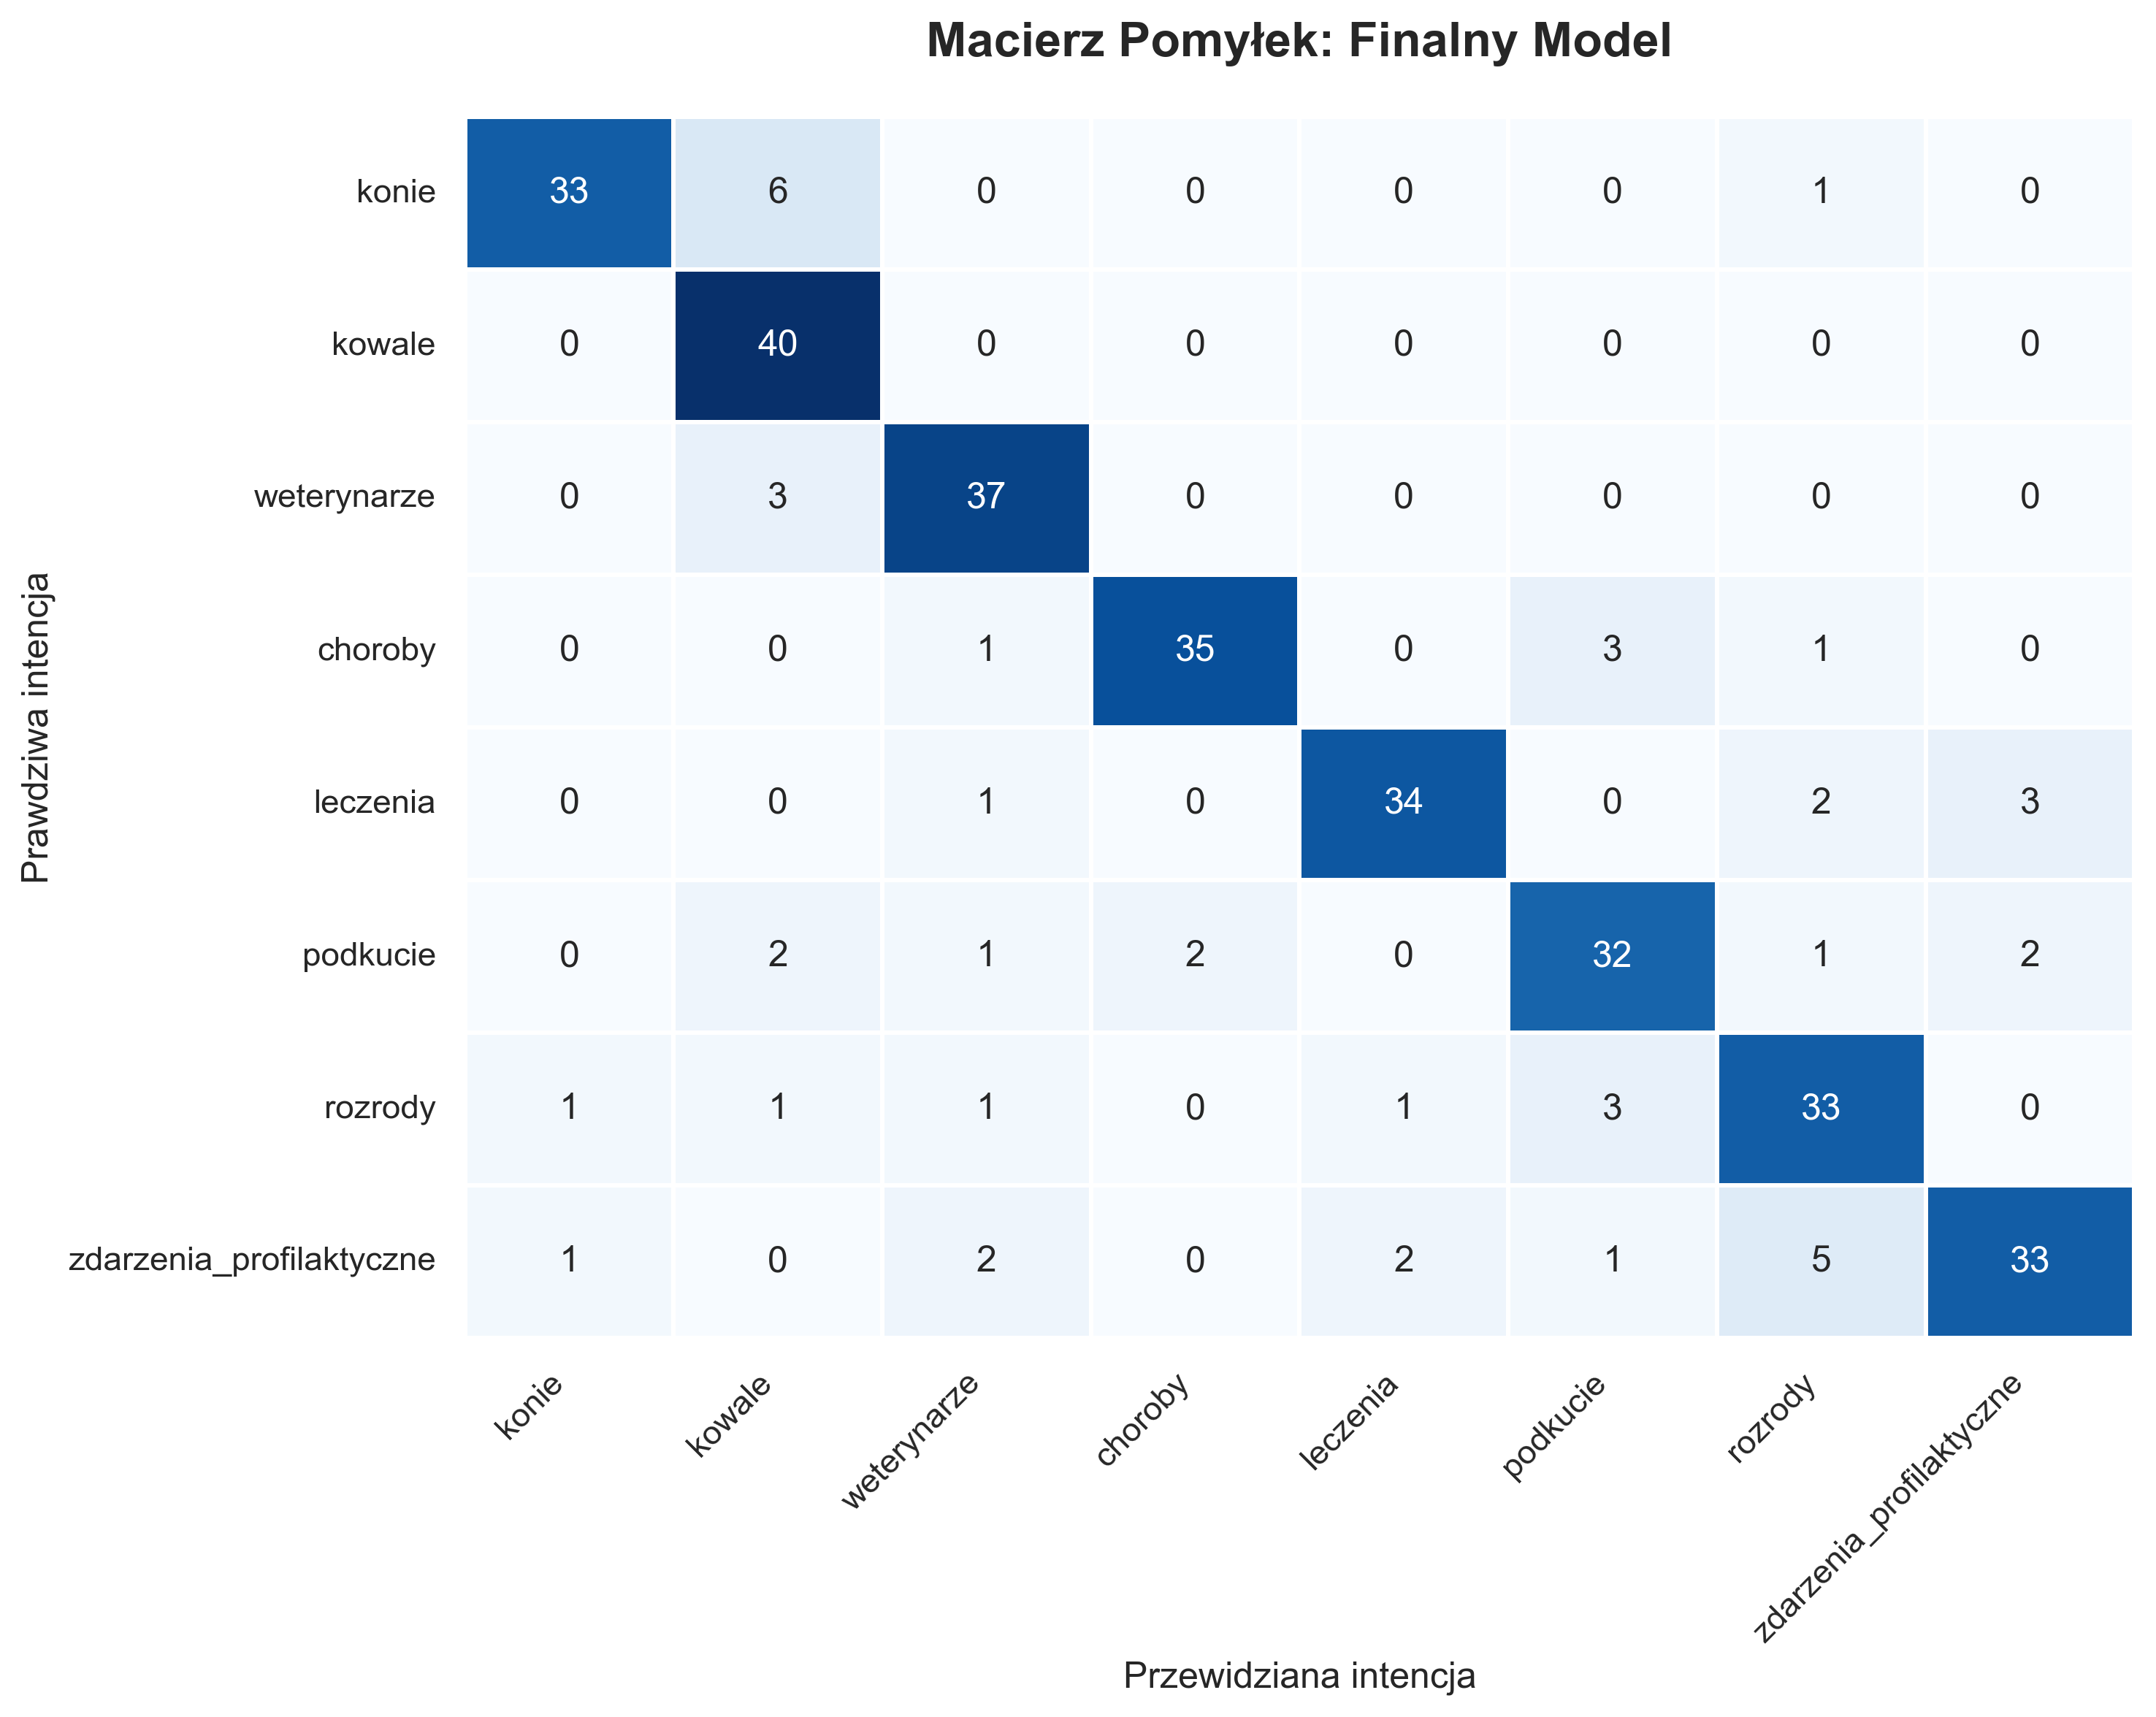
\includegraphics[width=0.9\textwidth]{public/macierz_pomylek.png} 
    \caption{Macierz pomyłek dla finalnego modelu w środowisku produkcyjnym.}
    \label{fig:macierz_pomylek}
\end{figure}

Szczegółowa inspekcja wyników prowadzi do następujących wniosków:

\begin{description}
	\item[Wysoka precyzja dla encji rzadkich:] Intencja \texttt{kowale} została rozpoznana bezbłędnie (40/40 przypadków). Sugeruje to, że słownictwo związane z tą profesją jest silnie dystynktywne w~przestrzeni wektorowej. Jednakże, zauważalna jest pewna asymetria – intencja \texttt{konie} była mylona z intencją \texttt{kowale} aż w 6 przypadkach. Może to wynikać z konstrukcji zdaniowych, gdzie imię konia występuje w bliskim sąsiedztwie słowa kluczowego oznaczającego specjalistę.
    
	\item[Nakładanie się kontekstów medycznych:] Największe rozproszenie błędów widoczne jest w~grupie intencji weterynaryjnych: \texttt{choroby}, \texttt{leczenia} oraz \texttt{zdarzenia\_profilaktyczne}. Jest to zjawisko oczekiwane, wynikające z naturalnego podobieństwa semantycznego (np. szczepienie jest zarówno procedurą medyczną, jak i elementem profilaktyki).
    
	\item[Interferencja profilaktyki i rozrodu:] Istotnym błędem jest mylenie intencji \texttt{zdarzenia\_\allowbreak{}profi\allowbreak{}laktyczne} z \texttt{rozrodami} (5 pomyłek). Wskazuje to na konieczność doprecyzowania bazy wiedzy o frazy rozróżniające opiekę nad źrebięciem (profilaktyka) od procesów hodowlanych w kolejnych etapach rozwoju proejktu.
\end{description}

\paragraph{Rekomendacje dla rozwoju systemu:}~\\
Analiza powyższych błędów wyznacza jasny kierunek dalszej optymalizacji. Przyszłe prace nad klasyfikatorem intencji powinny skupić się na:
\begin{enumerate}
    \item \textbf{Wzbogaceniu bazy wzorców o trudne przypadki:} Dodaniu do bazy wiedzy tych specyficznych sformułowań, które model obecnie myli. Pozwoli to systemowi lepiej nauczyć się subtelnych różnic między podobnymi klasami (np. skuteczniej odróżniać opisy koni od zapytań o kowala).
    \item \textbf{Klasyfikacji hierarchicznej:} Rozważeniu architektury dwuetapowej, gdzie model najpierw rozróżnia szerokie domeny (np. \textit{Operacje Cykliczne} vs \textit{Zdrowie}), a dopiero w drugim kroku precyzuje konkretną końcówkę. Pozwoliłoby to na zredukowanie szumu informacyjnego wewnątrz gęstego klastra intencji medycznych.
\end{enumerate}

Podsumowując, mimo wskazanych obszarów do poprawy, model osiąga stabilność operacyjną wystarczającą do wdrożenia w ramach sytemu \definicja{Moje Konie} i jego części \definicja{Asystenta NLP} 
